%!TEX root=../thesis.tex
\chapter{Technological stack} \label{cha:tech_stack}

There are a lot of technologies involved in this work. The whole system
architechture is composed of many different layers and the technological
stack under study is quite complex. Hence, this chapter aims at explaining
all the remarkable parts.


\section{FriWalk's architechture}
The whole system architechture can be divided into two main parts. One that
is completely platform agnostic and another one that is platform independent.
This distinction is due to the fact that, since the navigator application heavily
uses 3D graphics primitives, different operating systems handle them in different
ways.
\begin{figure}[!htb]\label{img:system_arch}
    \center{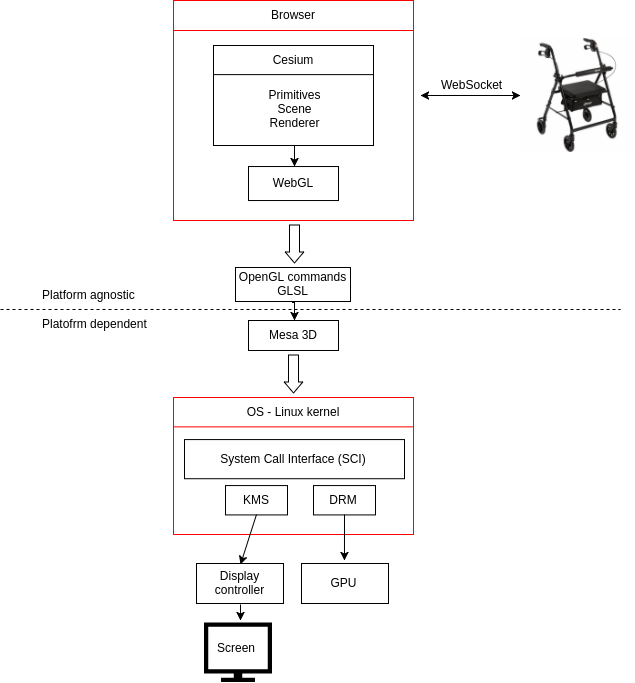
\includegraphics[width=0.6\linewidth]{system_architecture.png}}
    \caption{The FriWalk's system architecture.}
\end{figure}

As it is possible to see from Figure \ref{img:system_arch}, the first part includes
the walker assistant hardware, the browser running the
user interface (Google Chrome has been used in this study) and the component of
the OS which is responsible for implementing the OpenGL~\cite{woo1999opengl}
and the GLSL~\cite{marroquim2009introduction} standards. On the other hand,
the platform dependent part includes the 3D graphics driver (eg. Mesa 3D for
Linux) and the OS kernel (eg. the Linux kernel). In the specific case of the
Linux kernel, it is implements a System Call Interface (SCI) for interacting
with the Kernel Mode Setting (KMS)~\cite{linuxkms} and the Direct Rendering Manager
(DRM)~\cite{paul2000introduction}.


\subsection{Platform agnostic}
The 3D navigator application makes use of three pieces of information to move on
the map: the \emph{latitude}, the \emph{longitude} and the \emph{rotation}.
These three values is the
minimum amount of information needed for the navigator to behave correctly. Thus,
from an high-level point of view, the walker assistant hardware can be regarded
as the portion of the system that is able to provide such data. Mooreover, it can
guarantee that data are available for the navigator at a fixed interval over time
using a the WebSocket protocol~\cite{fette2011websocket}.\\
After receiving the data, the navigator properly moves the placeholder on the map.
This step can involves several operations, such as requesting a new tile for the
map, creating new 3D objects and so on. Consequently, the WebGL engine is responsible
for actually drawing the objects on the screen. How WebGL actually behaves
is described in Section \ref{sec:webgl}.\\
Finally, it is possible to say that the flow of information inside the platform
agnostic part of the system works as follows:
\begin{itemize}
    \item the FriWalk sends through a WebSocket the \emph{latitude}, the
        \emph{longitude} and the \emph{rotation} as a comma-separated string.
    \item the navigator running inside a browser receives the string, extracts
        the three values and uses them to build the objects needed to show the
        change on the screen.
    \item the framework powering the navigator application actually performs the
        WebGL function calls.
    \item the graphical engine implemented inside the browser translates the WebGL
        function calls into generic OpenGL and GLSL commands, which are directly
        feeded to the graphical driver.
\end{itemize}


\subsection{Platform dependent} \label{sec:platform_dependent}
This part of the system architechture highly depends on the operating system
running on the machine under test. In this work, a Linux-based OS has been used.
Therefore the description may not fit, fully or partially, to other operating
systems like Apple Mac OS X and Microsoft Windows.\\
The implementation of the OpenGL standard, the Mesa 3D Graphics Library. 
Graphics device drivers are implemented using two components: a User-Mode Driver
(UMD) and a Kernel-Mode Driver (KMD). The first can be seen as the interface
that can be used by other programs, while the second one directly interacts
with the KMS to set the display settings and with the DRM kernel subsystem
interfacing with the GPU(s). Starting from the 4.2 version of the Linux kernel,
multiple graphics drivers (eg. Mesa and AMD Catalyst) can share the same kernel
mode driver.


\section{Linux 3D graphics stack}
First it has to be underlined that we are referring only to the 3D part of the
graphics stack. This means that the window manager needs to ask the X11 server
only for the handle to a portion of the screen (i.e. the window).
3D graphics primitives do not need to any more interaction with the X11 server. This
is needed to bypass the client-server architecture of X11 which is not suitable for
real-time 3D graphics and rendering, since it would have introduced more layers
of communication, delays and unpredictability. This architecture is called
Direct Rendering Infrastructure (DRI)~\cite{paul2000introduction}; it is
necessary to overcome the issue where only the X server was allowed to access
the graphics hardware. Moreover, DRI is composed by a user-space and a kernel-space
(the DRM) part. This provides the building blocks that allow userspace applications
to directly access the graphics hardware in an efficient and safe way.
In addition, the DRM is a key component for the navigator application to achieve
hardware-accelerated 3D rendering and managing video memory in Mesa.

As briefly described in Section \ref{sec:platform_dependent}, the Linux graphics
stack is quite complex and consists of many different layers in different parts
of the OS. The main ones are: the Mesa 3D Graphics Library, the System Call
Interface, the Kernel Mode Setting and the Direct Memory Manager.\\
As it is possible to see from Figure \ref{img:linux_graphics_stack} DRM and 
display server belongs to the windowing system (eg. X11 or Wayland~\cite{wayland}) 
and it is not strictly necessary for applications directly using OpenGL function
calls.
\begin{figure}[!htb]\label{img:linux_graphics_stack}
    \center{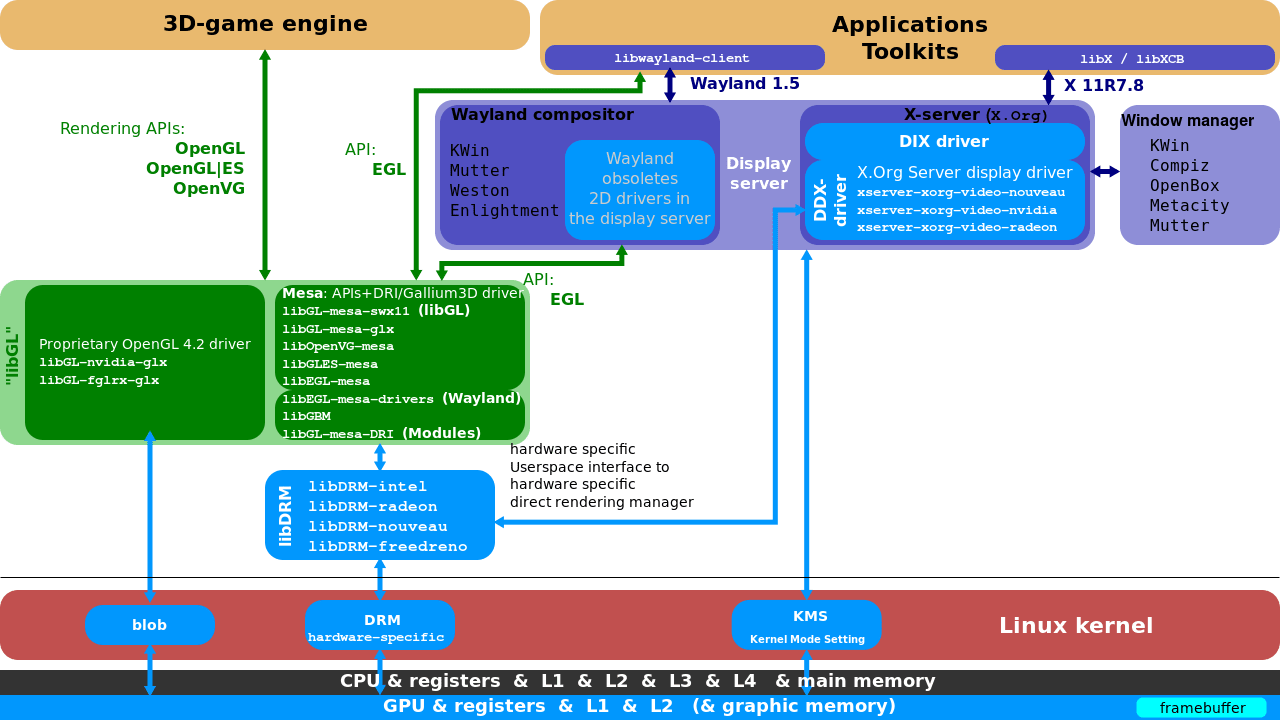
\includegraphics[width=0.75\linewidth]{linux_graphics_stack.png}}
    \caption{Illustration of the Linux graphics stack.}
\end{figure} 

Mesa is a free and open-source implementation of the OpenGL specification allowing
programs to output accelerated 3D graphics in the Linux environment. Fortunately,
DRI is conceived to run without the brokering of the X server, but it is still
needed to allocate to mesa a surface on the display to output to. Moreover, from
an high-level perspective the communication between Mesa and the GPU works by
exchanginc commands (eg. ``draw a point'') and data (eg. ``the coordinates of the
point and its color'') that are copied to a buffer of the graphics hardware.


\section{WebGL} \label{sec:webgl}
WebGL is a Javascript standard API for rendering 3D graphics within any compatible
desktop or mobile web browser\footnote{A compatibility table for all the most
common browsers can be found at the following link: \url{http://caniuse.com/#feat=webgl}.}
without any external program or tool. WebGL programs are composed of two parts
of code: some Javascript code, that can be mixed with any other part of a standard
HTML page and is executed by the browser, and some shader code, which is written 
in the OpenGL Shading Language (GLSL) and is executed by the GPU.
WebGL APIs and are exposed to the Javascript engine of the browser through the
HTML5 canvas element are based on the OpenGL for Embedded Systems (ES) technology,
which is a subset of standard OpenGL library. Moreover, this standard is both
royalty-free and open-source\footnote{The WebGL source code can be found on GitHub
at the following link: \url{https://github.com/KhronosGroup/WebGL}.}.

In the last few years a lot of frameworks and utility libraries have been developed
and the huge capabilities of these 3D graphics APIs become visible to everybody.
A lot of libraries have been built on WebGL to render scenes and 3D objects, such
as BabylonJS~\cite{babylon3d}, three.js~\cite{cabello2010three}, and 
Cesium~\cite{cozzi20113d} (see Section \ref{sec:cesium} for a more detailed description).
Moreover, there also has been a rapid emergence~\cite{parisi2014programming} of
game engines exploiting this technology like the Unreal Engine~\cite{games2007unreal}
and Unity~\cite{engine9unity}.

The reason why the 3D navigator developed in this work uses a framework built on
WebGL is that it is, at the time of writing, the only alternative to build real
3D graphics inside a browser. This choiche allows to write Javascript source
code to develop the application and, at the same time, to exploit the power of
a GPU using a framweork that takes care of implementing the shaders programs.
To be more precise, looking at the whole system architecture shown in Figure
\ref{img:system_arch}, WebGL is a technology that lie inside the browser
(in this specific case Google Chrome). The browser is the one responsible
for the communication with the actual implementation of OpenGL, which is Mesa
in this case study.



\section{Cesium framework} \label{sec:cesium}


\section{Goole Chrome's architechture}
